\documentclass[a4paper,12pt]{article}
\usepackage[colorlinks=false,pdfborder=000]{hyperref}
\usepackage[top=1.2in, bottom=1.2in, left=1.2in, right=1.2in]{geometry}
\usepackage[dvips]{graphicx,color}
\usepackage{times}
\usepackage{tikz}
\usepackage{fp}
\usetikzlibrary {snakes,arrows}

%%%%%%%%%%%%%%%%%%%%%%%%%%%%%%%%%%%%%%%%%%%%%%%%%%%%%%%%%%%%%%%%%%
\def\scale{0.7}
\def\half{0.5}
\providecommand{\blockage}[4]{%
    \fill[block] (#1,#2) rectangle (#3+1,#4+1);
}
\providecommand{\drawrowcol}[2]{
    % enumerate the row and column
    \FPset{\row}{#1}
    \FPadd{\row}{\row}{-1}
    \foreach \r in {0,...,\row}
        \node at (0-\half,\r+\half) {\r} ;
    \FPset{\col}{#2}
    \FPadd{\col}{\col}{-1}
    \foreach \c in {0,...,\col}
        \node at (\c+\half,0-\half) {\c} ;
}
\providecommand{\drawgrid}[2]{
    \draw (0,0) grid (#1,#2);
    \drawrowcol{#1}{#2}
}
\providecommand{\drawtwopin}[7]{
%#1= pin1 name #2,#3=pin1 location
%#4= pin1 name #5,#6=pin2 location
%#7= color
    \node[pins,#7]  (#1) at (#2 + \half, #3 + \half) {}; % pin-1
    \node[pins,#7]  (#4) at (#5  + \half, #6 + \half) {}  % pin-2
        edge[arrow] (#1);            % arrow
    %\node[above] at (#1) {$#1$}; % label
    %\node[above] at (#4) {$#4$}; % label
}
\providecommand{\drawthreepin}[9]{
%#1= pin1 name #2,#3=pin1 location
%#4= pin1 name #5,#6=pin2 location
%#7= pin1 name #8,#9=pin3 location
    \node[pins]  (#1) at (#2 + \half, #3 + \half) {}; % pin-1
    \node[pins]  (#4) at (#5  + \half, #6 + \half) {}  % pin-2
        edge[arrow] (#1);            % arrow
    \node[pins]  (#7) at (#8  + \half, #9 + \half) {}  % pin-2
        edge[arrow] (#1);            % arrow
}
%%%%%%%%%%%%%%%%%%%%%%%%%%%%%%%%%%%%%%%%%%%%%%%%%%%%%%%%%%%%%%%%%%
\begin{document}

\begin{figure}
\centering
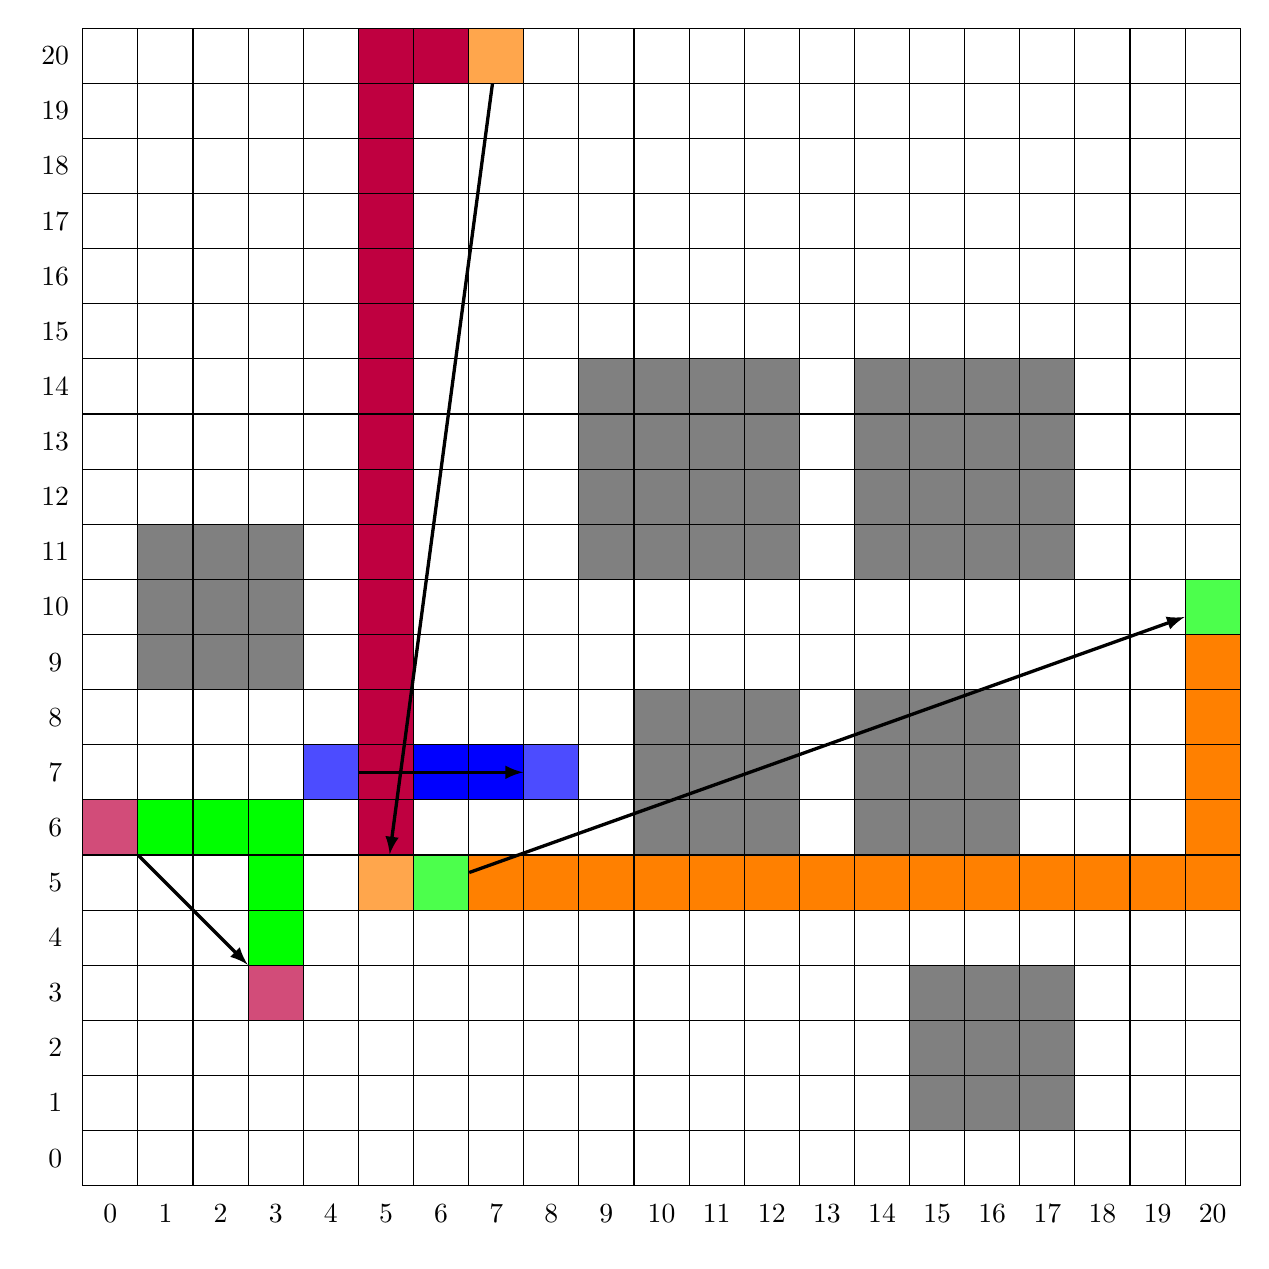
\begin{tikzpicture}[scale=\scale,
	%inner sep=1cm*\scale*\half,
	inner sep=0,
	minimum size=1cm*\scale,
	>=latex,
	pins/.style={rectangle,draw,fill=brown,font=\scriptsize},
	arrow/.style={->,very thick},
	block/.style={gray}]
	% define the row and column number
	\def \N{21}\def \M{21}
	% blockages
	% nets
	
\node[pins,blue] (net_0_4_7) at (4+\half,7+\half) {};
\node[pins,blue] (net_0_5_7) at (5+\half,7+\half) {};
\node[pins,blue] (net_0_6_7) at (6+\half,7+\half) {};
\node[pins,blue] (net_0_7_7) at (7+\half,7+\half) {};
\node[pins,blue] (net_0_8_7) at (8+\half,7+\half) {};
\node[pins,blue] (net_0_8_7) at (8+\half,7+\half) {};
\node[pins,blue] (net_0_8_7) at (8+\half,7+\half) {};
\node[pins,blue] (net_0_8_7) at (8+\half,7+\half) {};
\node[pins,blue] (net_0_8_7) at (8+\half,7+\half) {};
\node[pins,blue] (net_0_8_7) at (8+\half,7+\half) {};
\node[pins,blue] (net_0_8_7) at (8+\half,7+\half) {};
\node[pins,blue] (net_0_8_7) at (8+\half,7+\half) {};
\node[pins,blue] (net_0_8_7) at (8+\half,7+\half) {};
\node[pins,blue] (net_0_8_7) at (8+\half,7+\half) {};
\node[pins,blue] (net_0_8_7) at (8+\half,7+\half) {};
\node[pins,blue] (net_0_8_7) at (8+\half,7+\half) {};
\node[pins,blue] (net_0_8_7) at (8+\half,7+\half) {};
\node[pins,blue] (net_0_8_7) at (8+\half,7+\half) {};
\node[pins,blue] (net_0_8_7) at (8+\half,7+\half) {};
\node[pins,blue] (net_0_8_7) at (8+\half,7+\half) {};
\node[pins,blue] (net_0_8_7) at (8+\half,7+\half) {};

\node[pins,green] (net_3_0_6) at (0+\half,6+\half) {};
\node[pins,green] (net_3_1_6) at (1+\half,6+\half) {};
\node[pins,green] (net_3_2_6) at (2+\half,6+\half) {};
\node[pins,green] (net_3_3_6) at (3+\half,6+\half) {};
\node[pins,green] (net_3_3_5) at (3+\half,5+\half) {};
\node[pins,green] (net_3_3_4) at (3+\half,4+\half) {};
\node[pins,green] (net_3_3_3) at (3+\half,3+\half) {};
\node[pins,green] (net_3_3_3) at (3+\half,3+\half) {};
\node[pins,green] (net_3_3_3) at (3+\half,3+\half) {};
\node[pins,green] (net_3_3_3) at (3+\half,3+\half) {};
\node[pins,green] (net_3_3_3) at (3+\half,3+\half) {};
\node[pins,green] (net_3_3_3) at (3+\half,3+\half) {};
\node[pins,green] (net_3_3_3) at (3+\half,3+\half) {};
\node[pins,green] (net_3_3_3) at (3+\half,3+\half) {};
\node[pins,green] (net_3_3_3) at (3+\half,3+\half) {};
\node[pins,green] (net_3_3_3) at (3+\half,3+\half) {};
\node[pins,green] (net_3_3_3) at (3+\half,3+\half) {};
\node[pins,green] (net_3_3_3) at (3+\half,3+\half) {};
\node[pins,green] (net_3_3_3) at (3+\half,3+\half) {};
\node[pins,green] (net_3_3_3) at (3+\half,3+\half) {};
\node[pins,green] (net_3_3_3) at (3+\half,3+\half) {};

\node[pins,orange] (net_1_6_5) at (6+\half,5+\half) {};
\node[pins,orange] (net_1_7_5) at (7+\half,5+\half) {};
\node[pins,orange] (net_1_8_5) at (8+\half,5+\half) {};
\node[pins,orange] (net_1_9_5) at (9+\half,5+\half) {};
\node[pins,orange] (net_1_10_5) at (10+\half,5+\half) {};
\node[pins,orange] (net_1_11_5) at (11+\half,5+\half) {};
\node[pins,orange] (net_1_12_5) at (12+\half,5+\half) {};
\node[pins,orange] (net_1_13_5) at (13+\half,5+\half) {};
\node[pins,orange] (net_1_14_5) at (14+\half,5+\half) {};
\node[pins,orange] (net_1_15_5) at (15+\half,5+\half) {};
\node[pins,orange] (net_1_16_5) at (16+\half,5+\half) {};
\node[pins,orange] (net_1_17_5) at (17+\half,5+\half) {};
\node[pins,orange] (net_1_18_5) at (18+\half,5+\half) {};
\node[pins,orange] (net_1_19_5) at (19+\half,5+\half) {};
\node[pins,orange] (net_1_20_5) at (20+\half,5+\half) {};
\node[pins,orange] (net_1_20_6) at (20+\half,6+\half) {};
\node[pins,orange] (net_1_20_7) at (20+\half,7+\half) {};
\node[pins,orange] (net_1_20_8) at (20+\half,8+\half) {};
\node[pins,orange] (net_1_20_9) at (20+\half,9+\half) {};
\node[pins,orange] (net_1_20_10) at (20+\half,10+\half) {};
\node[pins,orange] (net_1_20_10) at (20+\half,10+\half) {};

\node[pins,purple] (net_2_7_20) at (7+\half,20+\half) {};
\node[pins,purple] (net_2_6_20) at (6+\half,20+\half) {};
\node[pins,purple] (net_2_5_20) at (5+\half,20+\half) {};
\node[pins,purple] (net_2_5_19) at (5+\half,19+\half) {};
\node[pins,purple] (net_2_5_18) at (5+\half,18+\half) {};
\node[pins,purple] (net_2_5_17) at (5+\half,17+\half) {};
\node[pins,purple] (net_2_5_16) at (5+\half,16+\half) {};
\node[pins,purple] (net_2_5_15) at (5+\half,15+\half) {};
\node[pins,purple] (net_2_5_14) at (5+\half,14+\half) {};
\node[pins,purple] (net_2_5_13) at (5+\half,13+\half) {};
\node[pins,purple] (net_2_5_12) at (5+\half,12+\half) {};
\node[pins,purple] (net_2_5_11) at (5+\half,11+\half) {};
\node[pins,purple] (net_2_5_10) at (5+\half,10+\half) {};
\node[pins,purple] (net_2_5_9) at (5+\half,9+\half) {};
\node[pins,purple] (net_2_5_8) at (5+\half,8+\half) {};
\node[pins,purple] (net_2_5_7) at (5+\half,7+\half) {};
\node[pins,purple] (net_2_5_6) at (5+\half,6+\half) {};
\node[pins,purple] (net_2_5_5) at (5+\half,5+\half) {};
\node[pins,purple] (net_2_5_5) at (5+\half,5+\half) {};
\node[pins,purple] (net_2_5_5) at (5+\half,5+\half) {};
\node[pins,purple] (net_2_5_5) at (5+\half,5+\half) {};

\blockage{9}{11}{12}{14}
\blockage{14}{11}{17}{14}
\blockage{1}{9}{3}{11}
\blockage{10}{6}{12}{8}
\blockage{15}{1}{17}{3}
\blockage{14}{6}{16}{8}
\drawtwopin{Dlt11_to_Dlt19}{8}{7}{Dlt11}{4}{7}{blue!70}
\drawtwopin{W}{20}{10}{Dlt11}{6}{5}{green!70}
\drawtwopin{Dlt14}{5}{5}{B1}{7}{20}{orange!70}
\drawtwopin{Dlt14}{3}{3}{Dlt07_to_Dlt14}{0}{6}{purple!70}
\drawgrid{\N}{\M}
	\end{tikzpicture}
      \end{figure}
      \end{document}
